\chapter{Evaluation}

This chapter is divided into the evaluation of the quantitative metrics captured by the implementation of this thesis and the network analysis of the graph, which can be generated out of the graph database and further analysed.

All previously described implementations were wrapped into individual docker containers, to first and foremost adopt "Infrastructure as Code", but also to use Kubernetes as scaleable infrastructure. The setup was running on a self hosted Kubernetes cluster using 5 baremetal machines, consisting of 2 master nodes and a total of 5 worker nodes, including the master nodes.

The graph database was occupying one of the 5 worker nodes, using a special taint to only schedule the database on this single node. Due to the usage of baremetal servers, and extra schedule taints, the local disk was directly mounted into the container to provide faster throughput compared to using a virtual disk. Each individual server provided 8 cores and 16 Gigabyte of memory. Typical cloud offers from Azure, AWS or GCP were not accessible.

The remaining implementations, e.g. Jenkins, the crawler and the proxy were all scheduled across the remaining 4 nodes.

The byte range of 0 bytes to 384.000 bytes were crawled within two weeks and no additional crawling was done afterwards, meaning the results are purely from one run, which covered all possible bytes that GitHub allows. The analysis took another two weeks and was done after the two weeks of crawling the results to not overload the graph database. The reasoning for this will be explained further down below.

\section{General Analysis}

Considering the crawler implementation one can compare the total amount of available "docker-compose" files that the GitHub API provides to the total amount the crawlers have crawled. As already described in the contribution about the crawler \todo{add reference to chapter}, the GitHub API has some limitations that affect the implementation as well. While providing a horizontally scaleable solution, which is only limited by the amount of GitHub tokens supplied, the GitHub API still has some nowhere described complications. This thesis and included test execution were all done under the terms of the GitHub Terms of Services, which states that the crawling of public data is only allowed for scientific works and require the results to be public \todo{quote TOS}. The TOS also states that the usage of the GitHub API is only allowed with a fair usage in mind, meaning one is not allowed to differ too much of the average usage of certain GitHub API routes. Not complying with those rule will likely result in a termination of ones account. During the data collection period, a total of three GitHub accounts were created with the sole purpose of crawling public data, which is only available with a valid GitHub account. Due to the excessive usage of the code search GitHub API route one out of three accounts received a so-called shadow ban. A shadow ban is a system to hide the fact that the user received a temporary termination. A shadow banned user can still use every GitHub API, but the results returned by the API are always empty even though they still conform the expected schema. GitHub as a provider of this free service does not provide any additional documentation about this system. It is not known at which point the account received the shadow ban, but it is to assume that this limitation was applied after the crawling period of two weeks, since the crawler still reported valid results back compared to two weeks later.

Besides this limitation the only other limiting factor was the 16 Gigabyte of memory for a graph database, which turned out to be not an issue by the memory itself, but the graph database had some blocking operations in the write process, which was heavily relied on. In a recent version this issue was fixed. This issue might have had an impact on the total amount of crawled files, since the database started to block any further insertions. To detect those issues a service called Sentry\footnote{https://sentry.io} was used, which sent alerts for not handled issues like the blocking of the database. This might have had an implication on the total amount of crawled files. The community edition of Grakn does not provide any Kubernetes manifests, thereby, manifests and settings have to be created by oneself, which likely results in a not entirely production ready setup, since the production ready setup with multi sharding is only reserved for the commercial usage.

In the following the actual amount of crawled entries will be compared to the possible and total amount of crawled items that the GitHub API returns. Both will be compared to each other by using a column chart.

\begin{figure}[H]
    \centering
    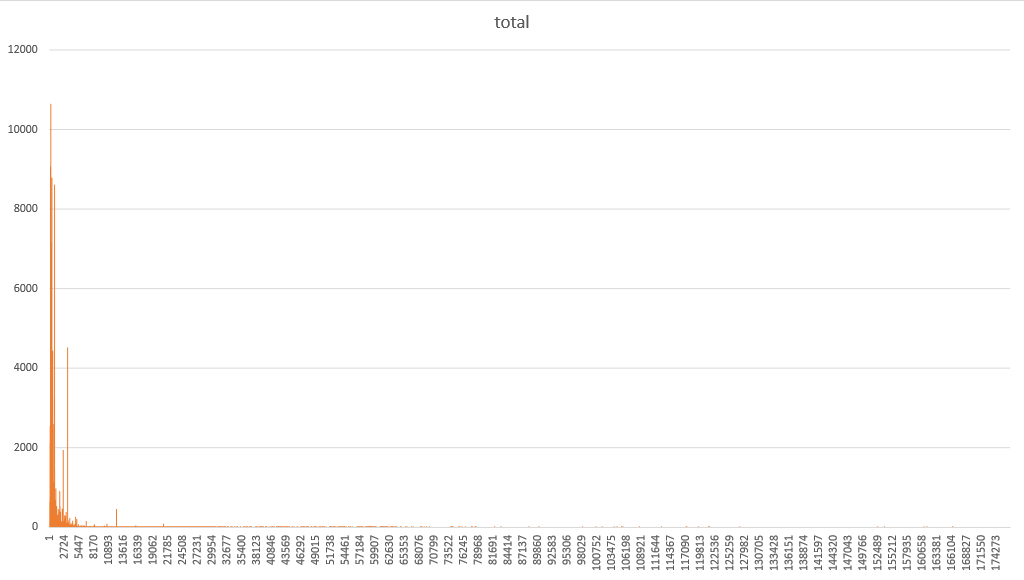
\includegraphics[scale=0.5]{graphics/stats_total.png}
    \caption{Chart representing the total amount of possible results using the GitHub API for the term "docker-compose"}
    \label{fig:stats_total}
\end{figure}

The chart \ref{fig:stats_total} represents the total amount of possible results for the term "docker-compose" using only the GitHub API. The Y-Axis represents the total amount of found occurrences and the X-Axis represents bytes. For this graphical representation the range from 0 to 175.000 was used, since between 175 Kilobyte and 384 Kilobyte are only an additional 200 results. There is a total of 1,1 million results in the chart, most of them clustered around the file size of 100 to 200 bytes, which can be explained due to "docker-compose" files being rather simple and short compared to other deployment scripts. 

\begin{figure}[H]
    \centering
    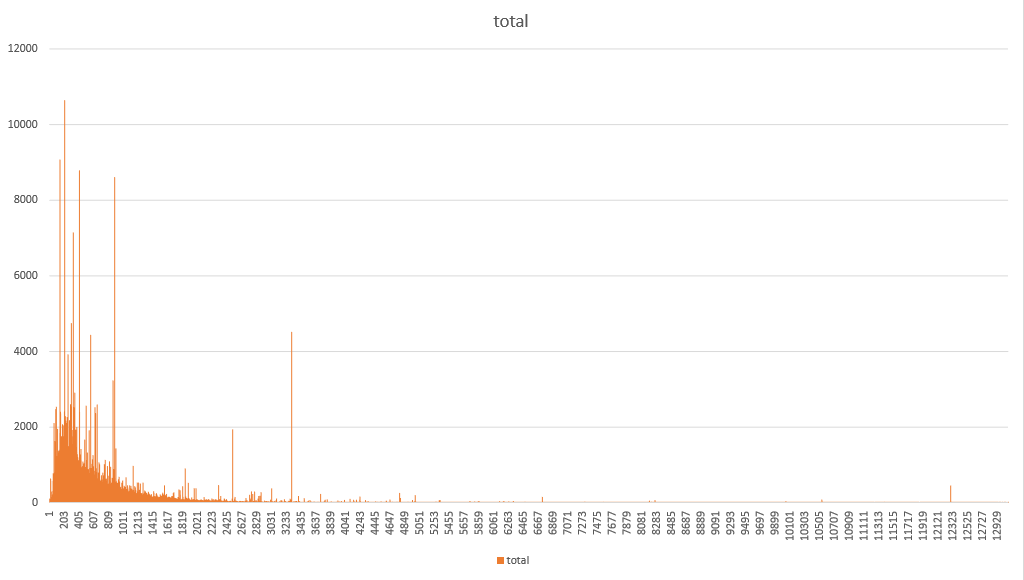
\includegraphics[scale=0.5]{graphics/stats_range.png}
    \caption{Cutout from \ref{fig:stats_total} for the range from 0 to 3000 bytes }
    \label{fig:stats_range}
\end{figure}

The cutout from the range 0 to 3000 bytes as seen in figure \ref{fig:stats_range} shows that the most files are in a range from 100 to 400 bytes and then slowly traverses towards 0, with as seen in figure \ref{fig:stats_total} occasional occurrences in a higher byte range. Both charts \ref{fig:stats_total} and \ref{fig:stats_range} represent the best case if GitHub would return more than a 1000 results for a single query and are both incomplete as well, since GitHub will only return the amount of found results till it receives a timeout. Meaning that running the same query twice would likely result in different results, as the API receives a timeout and returns all found results so far. This behaviour occurs as well when querying single pages, since GitHub only allows a maximal result of 100 entries. This could mean that for running one query on page 10 one could receive a 100 results and for another one close to 0, since the API received a timeout before. In case of this thesis this issue was dismissed, as the author has no influence on the actual implementation of GitHub and it could be mitigated by running the crawling process multiple times for the same bytes.

\begin{figure}[H]
    \centering
    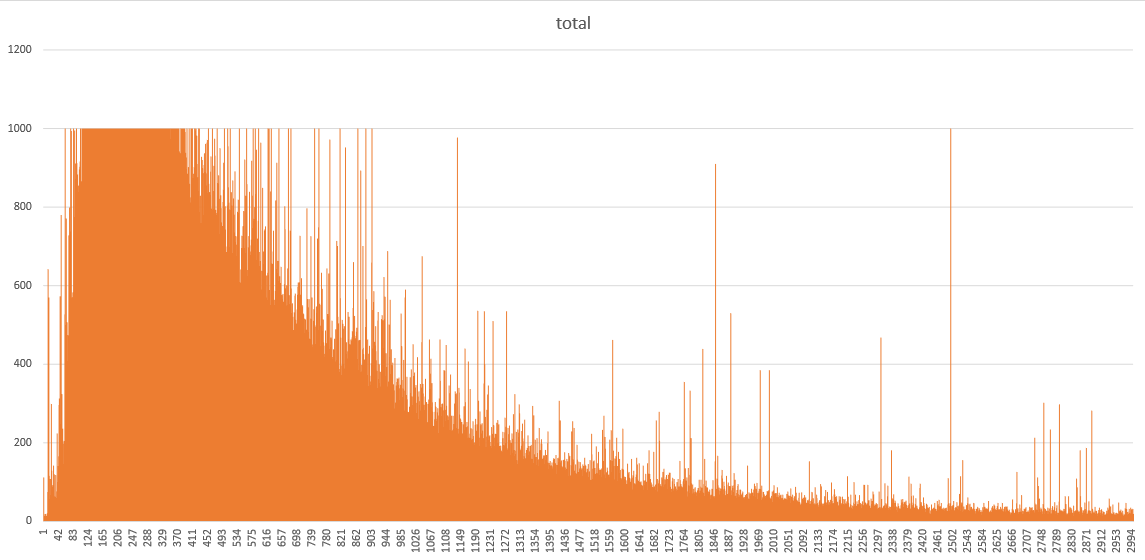
\includegraphics[scale=0.5]{graphics/stats_range_max_possible.png}
    \caption{Cutout from \ref{fig:stats_total} for the range from 0 to 3000 bytes, but a maximum of 1000 results }
    \label{fig:stats_max_possible}
\end{figure}

The chart in figure \ref{fig:stats_max_possible} shall represent the maximum amount of possible results, that can be crawled, since the GitHub API only returns a maximum of 1000 results for a single query. As explained prior for the chart \ref{fig:stats_range}, this does not mean that one will receive a 1000 results, since the GitHub API is nondeterministic.

Further on, the charts for the actual crawled data will be shown, which resulted in 140.000 valid deployments. Valid, since only parseable deployment files were inserted into the database, see \todo{add reference to the explanation in contribution} in the chapter about the implementation.

\begin{figure}[H]
    \centering
    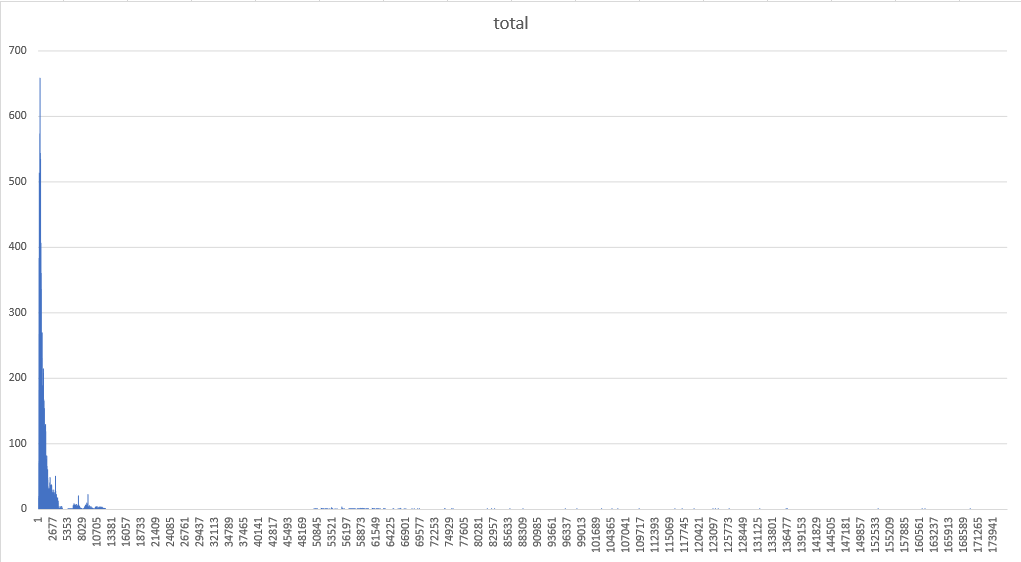
\includegraphics[scale=0.5]{graphics/deployment_stats_total.png}
    \caption{Chart representing the total amount of possible results using the crawler implementation for the term "docker-compose"}
    \label{fig:deployment_total}
\end{figure}

Comparing the figure \ref{fig:stats_total} and the figure \ref{fig:deployment_total}, one may notice a similar representation, which validates the overall implementation, since clusters for similar bytes were successfully crawled with occasional results in the higher byte area.
The chart \ref{fig:deployment_total} also shows that the maximum crawleable number of a 1000 results was never reached, which could be explained by either the nondeterministic behavior of the GitHub API or the blocking process of the database. On the other hand this could simply be explained by non parseable deployment scripts as well, since a lot of people have especially in the lower byte range scripts that are the bare minimum or contain syntactical issues, which cause the parsing to fail and at the same time render the file useless for the "docker-compose" executable as well, since it can not parse the file either.

\begin{figure}[H]
    \centering
    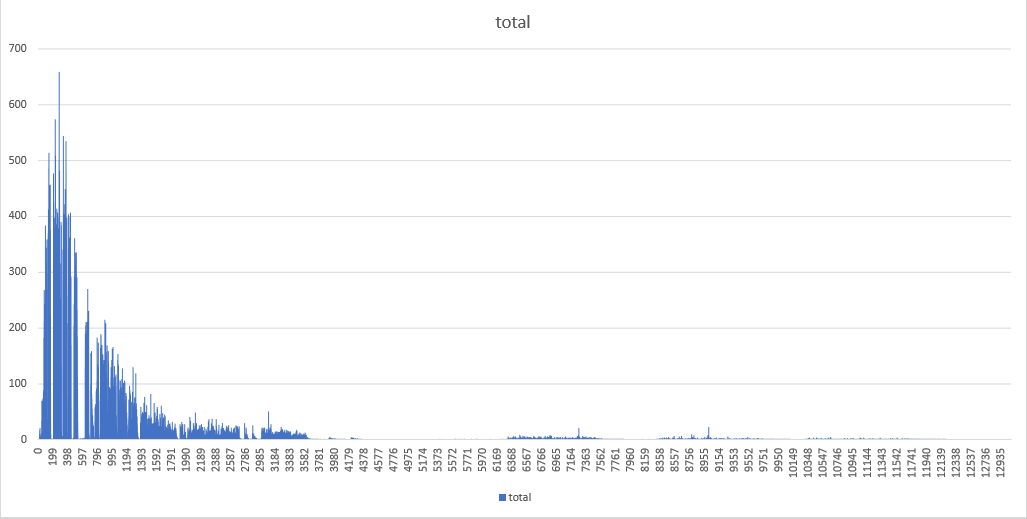
\includegraphics[scale=0.5]{graphics/deployment_stats_range.png}
    \caption{Cutout from \ref{fig:deployment_total} for the range from 0 to 3000 bytes}
    \label{fig:deployment_range}
\end{figure}

The chart \ref{fig:deployment_range} still resembles the chart \ref{fig:stats_range}, but it is visible that that the previously described shadow ban has occurred earlier than expected, since the chart \ref{fig:deployment_range} shows multiple spots where barely any results were returned, e.g. 161-201, 441-481 or 521-641, which mirror the system of a shadow ban. The implementation featured crawler windows, which consisted of a byte range that were individually assigned to each crawler, which in this case could have been assigned to the shadow banned account. During the execution period it was not visible that the account was affected, since it acted as expected and returned results according to the schema.

Overall the GitHub API returned a total amount of 940.000 possible crawleable entries, which can still differ in numbers when actually crawled for due to the way the GitHub API works. A total of 140.000 valid deployment scripts were inserted into the database, which represents 15\% of the total crawleable amount. Limiting factors were in this case the nondeterministic behavior of the GitHub API, the shadow ban system of GitHub and the blocking operations of the graph database. Except the nondeterministic behavior of the GitHub API all other issues can be mitigated for future work, by providing more valid GitHub tokens, which can be switched in case of shadow banned accounts and a more non-blocking graph database. Grakn already provided a patch to resolve the blocking issue, but in the non community edition the graph database can be scaled across multiple Kubernetes nodes as well, since the community edition does not provide any Kubernetes manifests and relied on the implementation of the author.

In total the graph database contains 4,2 million entries, which can be divided into roughly a million nodes, a million edges and two million attributes. Which can be further split down as follows:

\begin{table}[h!]
    \centering
    \begin{tabular}{ |c|c| }
    \hline
    Type & Amount \\
    \hline
         count & 4.279.664 \\
         attributes & 2.546.547 \\
         \hline
         nodes & 836.337 \\
         \hline
         user & 127.084 \\
         repository & 160.506\\
         deployment & 139.469\\
         service & 409.277\\
         \hline
         edges & 896.780 \\
         \hline
         own & 159.834 \\
         contain & 194.797 \\
         include & 404.736 \\
         depend & 137.412 \\
    \hline
    \end{tabular}
    \caption{Graph Database total counts}
    \label{graph_database_total_counts}
\end{table}

The approximately 400.000 services can be analysed further by having a look at the most used images and their versions. This will be divided into multiple tables with different categories, which are databases, programming languages and miscellaneous.

\begin{table}[h!]
    \centering
    \begin{tabular}{ |c|c|c| }
    \hline
    Image & Amount & Tags \\
    \hline
         postgres & 20074 & latest: 9132 | 9.6: 1106 | 9.5: 873\\
         mysql & 16103 & 5.7: 7353 | latest: 3516 | 5.6: 1054\\
         redis & 13817 & latest: 7110 | alpine: 2384 | 3.0: 350\\
         mongo & 11843 & latest: 7575 | 3.4: 451 | 3.2: 367\\
         mariadb & 3241 & latest: 1786 | 10: 221 | 10.1: 201\\
    \hline
    \end{tabular}
    \caption{Top 5 image counts for databases}
    \label{table_image_databases}
\end{table}

\begin{table}[h!]
    \centering
    \begin{tabular}{ |c|c|c| }
    \hline
    Image & Amount & Tags \\
    \hline
         node / javascript & 2346 & latest: 498 | 8: 136 | alpine: 111\\
         php & 1121 & apache: 114 | 7-fpm: 108 | fpm: 81 \\
         golang & 375 & latest: 94 | alpine: 24 | 1.8: 20 \\
         python & 353 & 3.6: 79 | latest: 39 | 3.7: 24\\
         java / openjdk & 325 & 8: 84 | latest: 31 | alpine: 16\\
    \hline
    \end{tabular}
    \caption{Top 5 image counts for programming languages}
    \label{table_image_languages}
\end{table}

\begin{table}[h!]
    \centering
    \begin{tabular}{ |c|c|c| }
    \hline
    Image & Amount & Tags \\
    \hline
         nginx & 8459 & latest: 4035 | alpine: 1453 | 1.13: 288\\
         rabbitmq & 3241 & 3-management: 851 | latest: 468 | management: 303\\
         hyperledger/fabric-peer & 2834 & latest: 836 | 1.4.0: 678 | 1.2.0: 212\\
         phpmyadmin/phpmyadmin & 2523 & latest: 2319 | 4.7: 38 | 4.8: 11 \\
         hyperledger/fabric-ca & 2105 & latest: 911 | \$IMAGE\_TAG: 376 | 1.2.0: 90\\
    \hline
    \end{tabular}
    \caption{Top 5 image counts for miscellaneous}
    \label{table_image_misc}
\end{table}

The table \ref{table_image_databases} describing the top 5 used databases, shows that most of those databases are relational databases, with only mongoDB and redis being non-relational. This leads to the assumption that relation databases are still much more popular compared to non-relational, especially taken that redis is an in-memory database.

\begin{figure}[H]
    \centering
    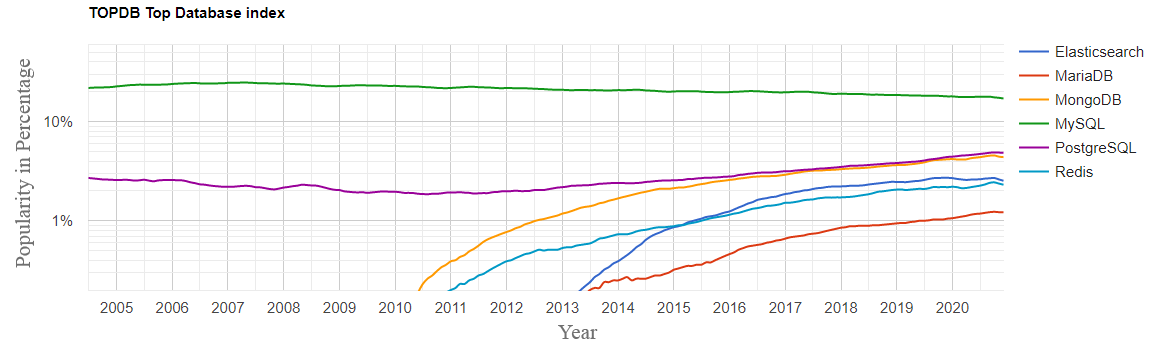
\includegraphics[scale=0.5]{graphics/databases_top_popularity_ranking.png}
    \caption{Most searched databases on Google Trends, which offer a docker image}
    \label{fig:databases_top_ranking}
\end{figure}

Taking a look at the chart \ref{fig:databases_top_ranking}, which describes the most popular databases searched for on Google Trends, for which publicly maintained docker images exist, it resembles the table \ref{fig:databases_top_ranking}, maybe not in the exact order, but in the listing of used databases.
Comparing the table \ref{table_image_databases} and the chart \ref{fig:databases_top_ranking} it is visible that they only resemble partly, which could be explained for various reasons. First of all the chart \ref{fig:databases_top_ranking} is based on Google Trends, which means solely on the amount of google searches, while the table \ref{table_image_databases} resembles the amount of usages in the particular use case of docker. Thereby, it can be said that some databases are preferably used in the context of docker, due to the way they work or the use case they are needed for. E.g. a lot of web applications are wrapped into docker images, due to which it makes a lot of sense to use such databases as postgres, mysql, mongoDB. Taking the table \ref{table_image_languages} into account it supports the assumption that docker images are often used in conjunction with web development, since Node.js and PHP are on number 1 and 2 with a big advance compared to the 3rd place.

\begin{figure}[H]
    \centering
    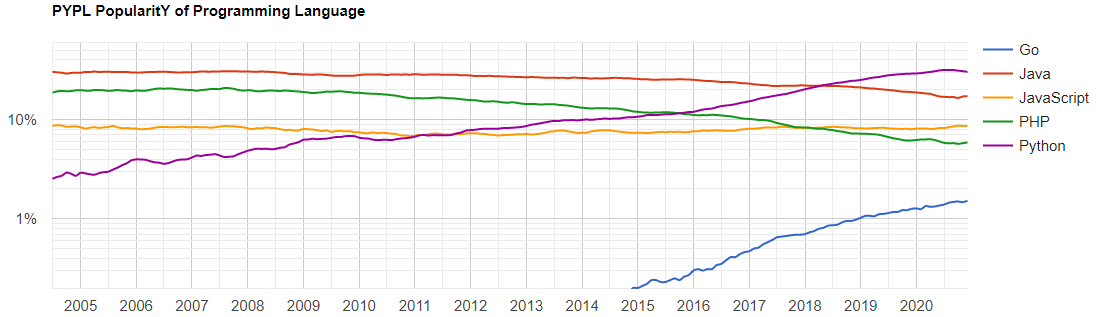
\includegraphics[scale=0.5]{graphics/languages_top_popularity_ranking.png}
    \caption{Most searched programming languages on Google Trends, which offer a docker image}
    \label{fig:databases_top_ranking}
\end{figure}

The table \ref{table_image_languages}, presents the most used programming languages with JavaScript and PHP far ahead of the remaining places. This can be simply explained, as earlier stated, that a lot of web development is done in conjunction with docker images and, therefore, "docker-compose" as it is often used to either have a local development environment or to run tests against such a predefined environment. Python on the other hand is distributed with most operating systems already, meaning someone that uses a Debian or Ubuntu images, or an image based on either one already has python included out of the box, due to which the amount of direct usages of python images is quite low.
The low usage of Java related images can be reasoned by the rather complex issues that Java brings along when used with Docker. The JVM was created before the introduction of cgroups, which Docker heavily relies on, due to which the JVM thinks it has access to the whole amount of CPU cores and memory on the machine, but in reality it is virtually limited to much less \todo{add source https://developers.redhat.com/blog/2017/03/14/java-inside-docker/}. This causes the Java container to crash more often due to memory issues, since the default is to use the all available resources. In the end this can be tweaked by supplying parameters to the JVM, but it is still not comparable to a native integration. A proper integration was done with Java 10 \todo{add source https://www.docker.com/blog/improved-docker-container-integration-with-java-10/}, which solves the resources issues. The majority of the java and openjdk images found are still using Java 8 with a share of 90\%.

Images with a lot of occurrences, but no unified category were summarized as miscellaneous in table \ref{table_image_misc}. Nginx is a reverse proxy, http cache or loadbalancer, thereby, it is interesting to see it so much in use with "docker-compose", since at least for local development it has no apparent advantage over directly binding an application to a local port. On the other hand, "docker-compose" files are compatible with "docker-swarm", which is Dockers take on container orchestration, which would possibly explain the amount of nginx images used.
For the remaining images it is interesting to see that things such as message brokers and blockchain technologies are so popular.

From the approximately 400.000 images covered the majority of images used the latest tag with 35\%, which is problematic, since the latest tag reduces the reproducibility. This reduces the validity of a "docker-compose" file, as depending on how old the file is the latest tag will most likely have changed already, especially for such things as databases or programming languages, where a major version can already break the implementation. The latest tag was covered in the best practices analysis as it should be avoided in favor of reproducibility.
Another 3,6\% are using alpine related images, while this is solely based on the image tag. The real value might be higher, since the tag depends on the users declaration, where popular docker image maintainers usually stick to the convention of declaring the base image in the tag.
For 3,1\% of all images a variable tag was used, which is an interesting approach as well, since it allows one to be flexible when it comes to choosing the image. As the Readme was not checked for those scripts, it might not be clear whether it is anyhow documented, which once more can have an impact on reproducibility.

Coming to the distributed analysis where Jenkins was used as a base system for running a predefined test for each "docker-compose" file. The tests were conducted for two weeks with a total amount of 60.000 executed tests. By the end a total of 18.000 scripts were successfully evaluated. The failure reasons of the other 42.000 tests can be viewed from different technical perspectives.

For once, public data was crawled and inserted into the database and GitHub repositories were either deleted or made private within this short time period, which accounts to a total of a 1000 repositories. The whole "docker-compose" file could have been saved in the database, but it only has limited further usage, since docker-compose files usually contain a build directive in the file, meaning without the repository the "docker-compose" file can't be executed and this already accounts for a sixth of the score and the vulnerability scan can not be executed in detail as well, which would be worth a third of the whole score. In the beginning, the proxy was missing a denylist causing the 1000 unavailable repositories to be rerun over and over again, but this was fixed during the analysis period.

Kubernetes was used as container orchestration and, as previously described, was set up on dedicated machines, which means the whole maintenance was included as well. A production ready setup was used for the 5 nodes cluster, but after running a total of approximately 20.000 pods no pods and, therefore, no further tests could be scheduled. It turned out that the etcd storage contained too many objects and started blocking the master nodes, which did not respond to any new requests. This caused the whole cluster to stall, since all requests received a timeout. This happened around the 40.000 mark again, resulting in a lot of aborted tests, as a lot of them had stalled.

Overall most of the Jenkins related issues can be mitigated by using managed Kubernetes clusters by e.g. Azure, AWS or GCP with dedicated node pools, which are only used by the CI system.

The score system, explained in the contribution \todo{add reference}, consists of in total 4 different criteria, with each a different significance for the final score. The first third is split into two sixth, since the criteria evaluated in there are of less importance in comparison to the remaining criteria. One sixth considers where a file can be executed or not. Another sixth covers the file length of the file, since the longer the file the more valuable it seems. One third covers the CVSS score, which considers the vulnerability of an image or in this case the vulnerability score of all included images. The last third covers "docker-compose" related best practices.

\begin{figure}[H]
    \centering
    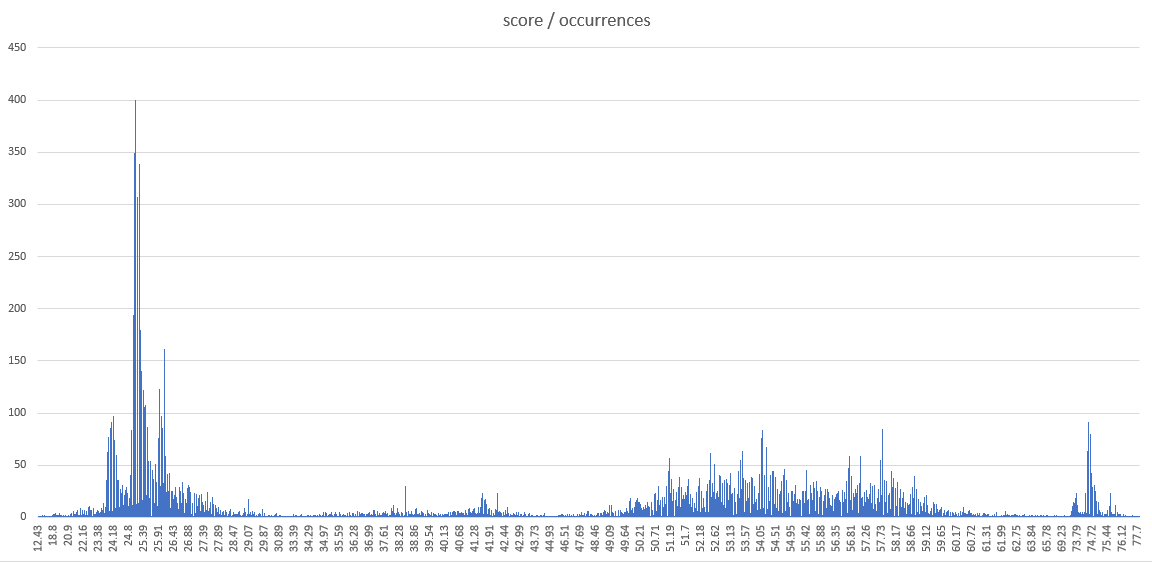
\includegraphics[scale=0.5]{graphics/deployment_score.png}
    \caption{Score distribution}
    \label{fig:deployment_score}
\end{figure}

The figure \ref{fig:deployment_score} shows the score distribution between 0 and 100, where 100 is the best possible score. The X-Axis represents the scores and the Y-Axis are the total amount of occurred scores. The chart shows that there are clusters around the score 24, 54 and 74, which could be explained through the split of the score in four criteria. Some of those criteria are more variable compared to others, e.g. executable is either a true or false and, thereby, contributes either fully or not at all to the score. Taking this fact into account, it's interesting to see that there is no score below twelve, which means that every evaluated deployment script fulfills at least parts of one criteria to the fullest. For the ones around twelve it is to assume that they are executable, since it counts as a sixth of the total score, but at the same time are short and vulnerable. Taking a look at the opposite side of the chart, there is nothing that fulfills a score of a 100, nor is a score close to it. This can be based on the issue of taking the file length too much into account as valuable source, as explained in the contribution part \todo{add reference to part} the file length of 300 as a reference for a "docker-compose" based deployment script might be too much and this unfolds in the chart, since there is a cluster around 74, which will fulfill almost all criteria to the fullest except the file length. For future work this could be changed to the file size, since the file size brings more value compared to the file length. Taking a look at the 180.000 crawled deployment scripts the median of the file length amounts to 22 and even taking the median of the upper part still amounts to 45, meaning that more than 75\% are smaller or equal to the file length of 45. On the other hand taking the file size into account it shows a median of 438 for the 180.000 scripts. This median would have been much more suitable for the score and could be used as a replacement for the file length. Nevertheless, since the file length only accounted for a sixth of the total score and in general has less significance for the value of its content, the score itself and the distribution shown in chart \ref{fig:deployment_score} are still valid and express the importance of the contents of a single deployment script.

\begin{figure}[H]
    \centering
    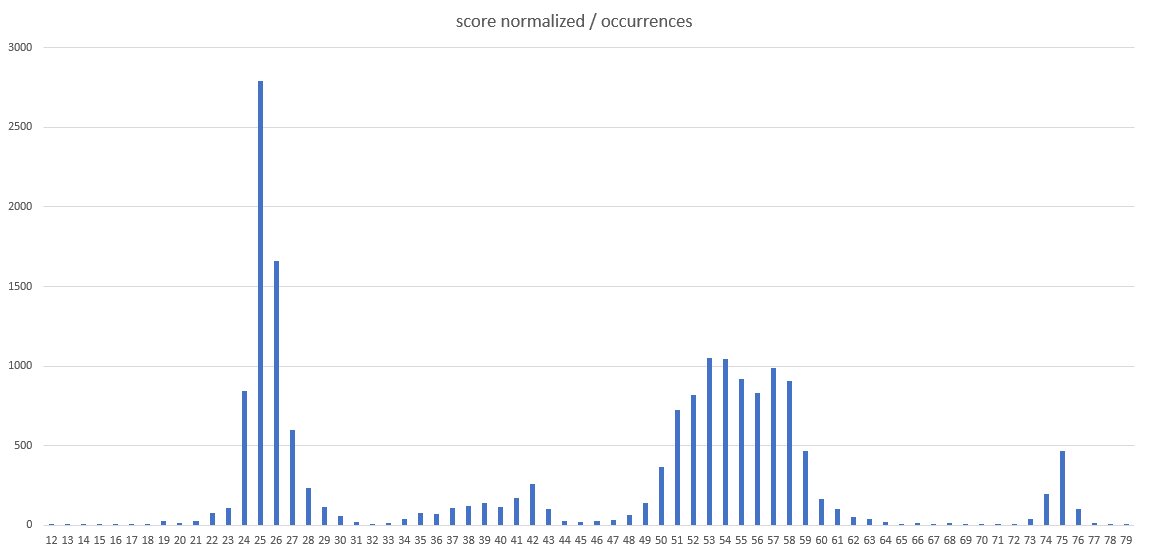
\includegraphics[scale=0.5]{graphics/deployment_score_normalized.png}
    \caption{Score distribution normalized}
    \label{fig:deployment_score_normalized}
\end{figure}

Taking a simplified look at the score distribution in the chart \ref{fig:deployment_score_normalized}, one can see a better picture of the score clusters. For the distribution between the score of 50 and 60 the amount of executable scripts amounts to 99\%, while the total amount of executable files amounts to 56\%. This cluster can be summarized as average but executable, as the deployment script is either fully vulnerable or fully following the best practices or, which is more likely, an average of both criteria.

The CVSS score is the most variable one and looking at the charts of \ref{fig:deployment_score} and \ref{fig:deployment_score_normalized} explain the values inbetween those previously mentioned clusters around the score of 24, 54 and 74.

The score gives an indication whether one script is more valuable compared to another. Still, the suggested scripts should be consumed with caution, since one might not know the contents of one image or the possible dangers of defining specific environment variables without enough care.
For future works the criteria of the file length should be replaced with the file size, as it brings more value compared to the length. The suggestion of using a Z-Score instead of a Min-Max normalization can be dismissed, since the goal of Z-Score normalization is to form the data into a normal distribution, which is not applicable for this type of data. Thereby, the Min-Max normalization is preferred, since the data requires to have the same scale, since one wants to compare across all available data with the same scale.

\begin{table}[h!]
    \centering
    \begin{tabular}{ |c|c|c|c| }
    \hline
    score & image & tag & base image \\
    \hline
         78,69 & linuxserver/letsencrypt & latest & alpine \\
         78,03 & myregistry/simplest-lab & simplestlb, simplestdb, simplestapp & alpine \\
         77,75 & try-webpack & dev & alpine\\
         77,70 & aporeto/apobar & crud & ubuntu \\
         77,53 & python & 3-alpine & alpine\\
         77,53 & traefik & latest & alpine\\
    \hline
    \end{tabular}
    \caption{Images with highest scores}
    \label{images_with_highest_score}
\end{table}

The table \ref{images_with_highest_score} represents the contents of the 5 deployment scripts with the highest score. While the table looks small, some of those images were used multiple times in the same file, making the "docker-compose" files rather complex.
Something that should stick out of the table \ref{images_with_highest_score} is the fact, that most images use alpine as a base image. Alpine compared to other distributions, used for docker, is more secure and simpler, due to the removal of a lot of standard libraries and executables. Due to the removal of such things the resulting image is much smaller and at the same time more secure, since the attack surface is shrinked quite a bit.
The one image that is using Ubuntu in this table is an assumption, since the Dockerfile is not publicly available, nor does the contents of the Docker image give any insights. The image does not contain any executable that one would assume, e.g. ls, echo, cd, shell, bash, and many more. The only thing possible is to gain access to the \$PATH by causing an error, but even this doesn't bring much more information than already known, except for the fact that "snap" is in the path. Snap is a package manager shipped out of the box with newer Ubuntu versions, thereby the assumption of Ubuntu. Nevertheless, this image is much more secure than a default Ubuntu image and shows how to properly secure ones container even against reverse engineering.
Besides alpine as base image, busybox is used quite often as well, since it combines a lot of utilities into a single executable and is perfect for running simple scripts or in the context of Kubernetes as initialization container. Due to its limitied capabilities it's quite secure as well, since there is barely any attack surface.

Due to the popularity tables \ref{fig:databases_top_ranking}, \ref{table_image_languages}, and \ref{table_image_misc} one can now analyse common connections to other used images. First of all, which programming languages are often used in conjunction with e.g. databases or even message queues.
For this the first pick is Node.js, since it had the most occurrences in this category. The table \ref{node_commons} shows the 5 images with most occurrences in conjunction with Node.js. MongoDB being the most common database used, which is often used in conjunction with Node.js, especially for quick prototyping of projects, since a schema doesn't have to exist from the beginning of the project and can be extended over multiple iterations without having to migrate the data all the time. Nginx as reverse proxy or loadbalancer is commonly used for web development, may it be for local development or for deploying it in Docker Swarm. The type of database used with Node.js always depends on the type of project on is working on, thereby, it makes sense to see mysql and postgres as well, especially there were often used than mongoDB according to the table \ref{fig:databases_top_ranking}. Redis in conjunction is often used as session storage, since it is an in-memory database.

\begin{table}[h!]
    \centering
    \begin{tabular}{ |c|c| }
    \hline
    image & occurrences \\
    \hline
         mongo & 363 \\
         nginx & 337 \\
         mysql & 289 \\
         postgres & 241 \\
         redis & 174 \\
    \hline
    \end{tabular}
    \caption{Common images in conjunction with Node.js}
    \label{node_commons}
\end{table}

The second pick is PHP, as it was the second most used programming language as stated in table \ref{table_image_languages}. The most used image in conjunction with PHP is nginx for the same reasons as described in Node.js. PHP and Node.js are both programming languages or rather frameworks used for web development, especially for the backend. The most used database according to the table \ref{php_commons} is mysql, which is a relational database. Those are often used in conjunction with PHP, which would also explain the numbers in regards to mariaDB. MongoDB was only used 11 times in conjunction with PHP. PhpMyAdmin is an administration tool for mysql databases, which explains the high usage as well, since mysql is the dominant database for PHP.

\begin{table}[h!]
    \centering
    \begin{tabular}{ |c|c| }
    \hline
    image & occurrences \\
    \hline
         nginx & 432 \\
         mysql & 287 \\
         phpmyadmin & 97 \\
         mariadb & 95 \\
         redis & 56 \\
    \hline
    \end{tabular}
    \caption{Common images in conjunction with PHP}
    \label{php_commons}
\end{table}

So far a lot of individual images were covered, but one common usage of "docker-compose" files is to build an image on execution. The number of images build during execution are 24.146, where the contents are unknown, since they are described in a Dockerfile. Nevertheless it is still an interesting factor, due to the circumstance of not knowing parts of the implementation. The most common images in conjunction with self build images are databases, followed by nginx. Other interesting mentions are alpine with 517 and rabbitmq with 281 usages. The top 5 used images in conjunction can be seen in table \ref{self_build_commons} and mostly resemble databases.

\begin{table}[h!]
    \centering
    \begin{tabular}{ |c|c| }
    \hline
    image & occurrences \\
    \hline
         postgres & 4380 \\
         redis & 2666 \\
         mongo & 2356 \\
         mysql & 2076 \\
         nginx & 669 \\
    \hline
    \end{tabular}
    \caption{Common images in conjunction with self build images}
    \label{self_build_commons}
\end{table}

In conclusion, the most used databases are relational and the most used programming languages are used for web development. Thereby, one can conclude that in particular "docker-compose" is used a lot in terms of web development. This being supported by the most used miscellaneous image, which was nginx a reserve proxy and loadbalancer. The majority of images uses the latest tag with approximately 35\% of all images, which should be avoided, since it hampers the possibility to successfully execute the same file again after a long period. Alpine images only contributing with 3,6\% is another indicator for users to reconsider the security of their images.

\section{Network Analysis}

The following will cover the network analysis, since a graph database was used, which can in return be used to generate a graph out of the data and analysed according to social metrics. While GitHub is not a social network in a classical sense, a lot of social aspects are still present, since users can fork repositories or follow the same tutorial, due to which it can happen that the "docker-compose" file contains the same contents and thereby the same SHA hash. If the hash is the same for a deployment users and their repositories will be linked respectively, likely causing clusters.
For the graph visualization the program Gephi\footnote{https://gephi.org/} was used, which offers various implementations of algorithms already out of the box. The graph layout was done with the OpenOrd implementation, which Martin et al. describe in their paper as suitable for large graphs with a focus on both local and global structure\cite{openOrd}. The OpenOrd layout focuses bigger communities around the center of the graph and towards the edge of the graph smaller communities are arranged.

\begin{figure}[H]\centering
\begin{tikzpicture}[spy using outlines={circle,red,magnification=3,size=5cm, connect spies}]
    \node { \includegraphics[scale=0.06]{graphics/graph_modularity_v3.png} };
    \spy on (-0.15,0.95) in node [right] at (4,1.5);
\end{tikzpicture}
    \caption{Graph showing communities with more than a hundred members}
    \label{fig:graph_communities}
\end{figure}

The graph \ref{fig:graph_communities} presents all data that can be useful for analysing social metrics. This includes all entities for users, repositories and deployments, coming to a total of 427.045 nodes and 354.629 edges. The graph is directed, since a relation is always one sided, meaning a user owns a repository, which includes a deployment. In the figure \ref{fig:graph_communities} all communities with more than a 100 members are colorized, which comes to a total of 102 communities of a size bigger than 100. For this the algorithm described by Blondel et al. was used, who describes their algorithm as accurate and fast even for big networks and mostly only limited by the amount of memory available \cite{Blondel_2008}. The zoom focuses on the two biggest communities, in the colors blue and orange. The orange community comes to a total of 2773 members and the blue community to 2866 members. The bigger one of these, the blue community, comes to a total of 971 users with 1353 repositories and 542 deployments. The deployment that connects most of the users is embedded in a repository\footnote{https://github.com/ajeetraina/docker101} about how to learn docker and none of those repositories being forks of the original, this connects already 270 users. The deployment script with the highest score in this community describes an nginx alpine image with a total score of 75,55.
The second biggest community contains 795 users with 1197 repositories and 781 deployments. With 302 connections the deployment script is embedded into a repository\footnote{https://github.com/souravs93/first-program} about Hyperledger, which was mentioned as well in the table \ref{table_image_misc} about the most used docker images in the category miscellaneous. A score of 74,91 is the biggest one for this community, describing a node alpine based "docker-compose" file.

\begin{figure}[H]
    \centering
    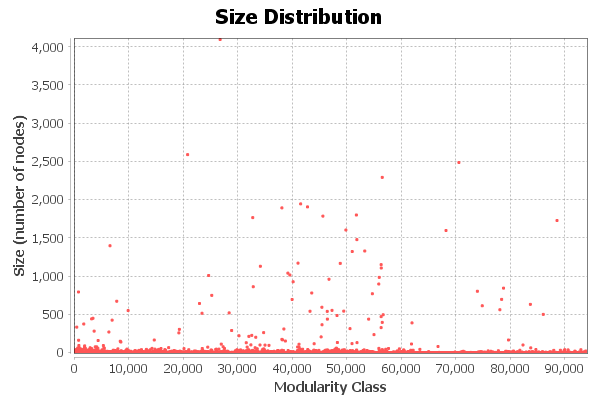
\includegraphics[scale=0.8]{graphics/modularity_stats.png}
    \caption{Community distribution}
    \label{fig:community_distribution}
\end{figure}

The figure \ref{fig:community_distribution} shows the distribution of all communities and their sizes. The X-Axis states each individual community, here called Modularity Class, and the Y-Axis represents the size. As can be seen the majority of all communities is far below the size of 200 and as states earlier only a 102 communities are bigger than the size of 100. There is a total amount of 94.072 communities with a modularity score of 0,977. Blondel et al. describes in their paper that the higher the modularity score the higher is the density of communities\cite{Blondel_2008}. The average nodes per community comes to the size 4, since even a single user with repository and deployment is already a community, but for this paper bigger communities as seen in the figure \ref{fig:graph_communities} are more interesting.

\begin{figure}[H]\centering
\begin{tikzpicture}[spy using outlines={circle,red,magnification=3,size=7cm, connect spies}]
    \node { \includegraphics[scale=0.06]{graphics/graph_type.png} };
    \spy on (1,-1) in node [right] at (3,1.5);
\end{tikzpicture}
    \caption{Graph according to their type and degree}
    \label{fig:graph_types}
\end{figure}

The graph presented in \ref{fig:graph_types} is ranked according to the degree of a node, with the setting the higher the degree the bigger the node. This shall visualize more important nodes compared to others. The coloring scheme is adjusted to the type of node with blue being repositories, orange being deployments and green being users. Looking at the overall graph it visualizes that in general deployments have a higher degree and are thereby linked more, which can also be explained by using the deployment script hash for linking the same nodes together. Nodes with a high degree and of type user are sort of super users with a lot of repositories and deployments. While a big node of type repository visualizes a super repository that contains a lot of deployment scripts.
The zoom in the figure \ref{fig:graph_types} shows the biggest repository, user, and deployment script.
1614 deployment script does the repository contain and is by far the biggest one with 1308 deployment scripts than the second biggest repository. Further analysing the repository it shows that the GitHub repository\footnote{https://github.com/vsplate/dcenvs} is used as a data store for a website\footnote{https://www.vsplate.com/} that allows to run any "docker-compose" file remotely, thereby, explaining the high degree, since it is used as an active store for "docker-compose" files.
The biggest deployment script has 881 repositories linking to it and is embedded in a Github repository\footnote{https://github.com/knex/knex}, which is a popular implementation of an SQL query builder for Node.js.
GitHub sees users and organisations as the same entity and, thereby, the user\footnote{https://github.com/crowdbotics-apps} with the highest degree has 459 repositories and is a service that offers a construction kit for apps, by offering a web service, that allows doing so in the web browser. This would explain the high degree of repositories, since each individual app is its own repository.

\begin{figure}[H]\centering
\begin{tikzpicture}[spy using outlines={circle,red,magnification=3,size=5cm, connect spies}]
    \node [opacity=0.7] { \includegraphics[scale=0.06]{graphics/graph_type.png} };
    \node [opacity=0.6] { \includegraphics[scale=0.06]{graphics/graph_modularity_v3.png} };
    \spy on (-0.15,0.95) in node [right] at (4,1.5);
\end{tikzpicture}
    \caption{Figure \ref{fig:graph_communities} and figure \ref{fig:graph_types} overlayed}
    \label{fig:graph_merged}
\end{figure}

Overlaying both figures \ref{fig:graph_communities} and \ref{fig:graph_types} in figure \ref{fig:graph_merged} shows that communities are fairly often gathered around nodes with a high degree. While none of the biggest users, repository, or deployment scripts are in the biggest communities. It is also visible that the entities in those communities are much smaller compared to other communities, which leads to those communities being sparsely connected, since there is not one main anchor to connect all nodes of the community. Another feature that is visible is, that outside of the core all remaining smaller communities are visible and none of those have a high degree node connecting them. The majority of the communities are small and surrounding the core of approximately a 100 bigger communities.

The so-called small world problem can be seen in this graph as well if the graph is interpreted as directed graph. Stanley Milgram describes in the paper about the small world problem, that if one takes two random people out of the population of the United states, how long would be the chain of mutual acquaintances? \cite{SmallWorld}. To figure out whether a small world problem exists, one uses the average path length, since it describes the average path from two nodes within a community. The graph in figure \ref{fig:graph_communities} has a diameter of 2 with an average path length of 1,3. This can be explained by the communities always being connected by at most 2 hops between nodes, since the system consists of only 3 types of nodes and the deployment script being the most connected one. While the small world problem is applicable within communities, it is not applicable for the whole graph, as the graph is not well connected overall. Another indicator that the small world problem does not exist in the overall graph is the average clustering coefficient, which Watts describes in his article about the "Collective dynamics of 'small-world' networks"\cite{Watts1998Collective} how complete a node's neighborhood is, also often called a clique. In this case the average cluster coefficient is 0, since there are no connections between users or even between other repositories.

To summarize, the presented graph, derived by the data crawled from GitHub, is not a social graph in a typical way, but still shows interesting characteristics, which are worth analysing. While the general analysis brought forward quantitative metrics based on the crawled data, about e.g. the top used images and their versions, the graph analysis brought forward interesting graphical interpretations. It showed big communities, which can be narrowed down to specific deployment scripts and, thereby, the origin of those and how users across GitHub are consuming those, e.g. by trying to learn more about Docker or the implicit popularity of a NPM library. On the other hand, one can identify repositories, which are used as data storage to run a commercial product around it, in this case a "docker-compose" as a service. Even users and their business ideas are identifiable, in the case of the app builder, which uses GitHub to house their applications. While the main idea of the graph database is to use it to recommend "docker-compose" files according to user defined metrics, it is still interesting to see how "docker-compose" is used across the community and especially around GitHub as a product itself. This would not have been possibly without the additional graph analysis and the possibility of visualizing such things. Further on this could be extended in the future to recommend other interesting metrics, such as tutorials or libraries, since an implicit popularity rating can be derived by the amount of usages across the GitHub community. Although this is a manual process, it can be further automated by analysing the user/organizations profiles itself or the repositories the files are hosted in.
Future work might experience limitations due to Dockers transition into sustainability, since docker announced in August an image retention policy \todo{cite https://www.docker.com/blog/scaling-dockers-business-to-serve-millions-more-developers-storage/}, which will automatically delete images created by free accounts if they have not been used for 6 months. From a business perspective it makes a lot of sense, since they try to acquire more business customers, which was never really necessary for Docker, as they offered all necessary services for free. As of December 2020 the introduction of the image retention policy was moved to mid 2021. Another limiting factor from Dockers side is the introduction of limiting the amount of docker pulls per 6 hours as a free account, which according to their pricing is 200 pulls per hour \footnote{https://www.docker.com/pricing}. The distributed analysis heavily relies on the docker hub, since most images are hosted on this platform. Therefore, the distributed analysis, depending on the load, reaches that number within an hour, which essentially renders the process useless for the next 5 hours. Overall this can be mitigated by subscribing to their service, which they call road to sustainability \todo{cite https://www.docker.com/blog/dockers-next-chapter-our-first-year/}, there is as of December 2020 no additional offer for educational purposes.
Besides that, the most limiting factors described in this evaluation can be mitigated, by either running the project on a more reliable infrastructure, e.g. managed Kubernetes by any cloud service, and through providing more valid GitHub tokens to avoid shadowbans. This could possibly achieved as well by reaching out to GitHub and declaring it as educational purpose, as long as the results are published publicly.
Research establishments such as the Fraunhofer-Allianz Cloud Computing\footnote{https://www.cloud.fraunhofer.de/} could pick up this topic and further develop it in regards to cloud optimization of deployment scripts with the aid of machine learning. For this purpose additional deployment scripts like Kustomize or Ansible should be integrated.


%Second most important chapter. Verifies the theses defined in the previous chapter. Tries to evaluate and analyze the contribution in qualitative or quantitative terms. Ends with a discussion. Approximately 20 to 30 pages. Can be split into multiple chapters.

% Hier solltest du die limitations deiner Contirbution versuchen zu analysieren. Dies können quantitative sachen sein, wie die limitationen des crawlers wie oft gecrawlet werden kann über github api und wie oft dann andere ergebnisse rauskommen. andere sachen wären zB ob der von dir erstellte score "qualitativ gut" IaC bewerten kann. Für diese unterschiedlichen Punkte sollten folgende Unterpunkte folgen:
%a) Evaluation Setup: hier wird der versuchsaufbau und die durchführung beschrieben. welche größen werden zB gemessen sollte auch beschrieben werden. Womit wird vielleicht das ergebnis verglichen?
%b) Results: Darstellung der Ergebnisse und Beschreibung der Ergebnisse
%c) Discussion: Bewerte die Ergebnisse und ordnete sie ein.
%Am Ende des Kapitels sollte dann eine summary kommen, was der leser gelernt haben soll und welche fragen noch offen geblieben sind für future work und welche forschungsrichtungen man diese arbeit weiter entwickeln kann.
